%----------------------------------------------------------------------------
\chapter{\bevezetes}
%----------------------------------------------------------------------------

\section{Motiváció és háttér}

\lettrine{E}zt a projektet nem a tanszéki diplomamunkatémák listáján találtam, hanem én kerestem hozzá konzulest. Szeretném ezért először megemlíteni a személyes motivációmat, és érdekeltségeimet vele kapcsolatban. Mint a legtöbb reál beállítottságú fiú, engem is fiatal korom óta érdekel a technológia, a járművek, a gépek, vagy a fegyverek. Ezek közös metszéspontja a haditechnológia, ami általában jóval fejlettebb, mint amivel a civil életben találkozhatunk. Ez az érdeklődés megmaradt kamaszkoromra is, amikor a videojátékok által új ingerként értek a \textsl{Team Fortress 2}-ben és a \textsl{Portal}-ban lévő ún. \textbf{Sentry Gun}-ok. \\[5mm]



\begin{figure}[h!]
	\centering
	\begin{minipage}{.5\textwidth}
		\centering
		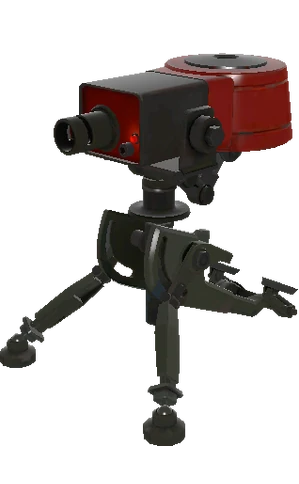
\includegraphics[width=0.8\linewidth]{irod_tf2} 
		\caption{TF2 Sentry Gun \cite{tf2}}
		\label{fig:irod_tf2}
	\end{minipage}%
	\begin{minipage}{.5\textwidth}
		\centering
		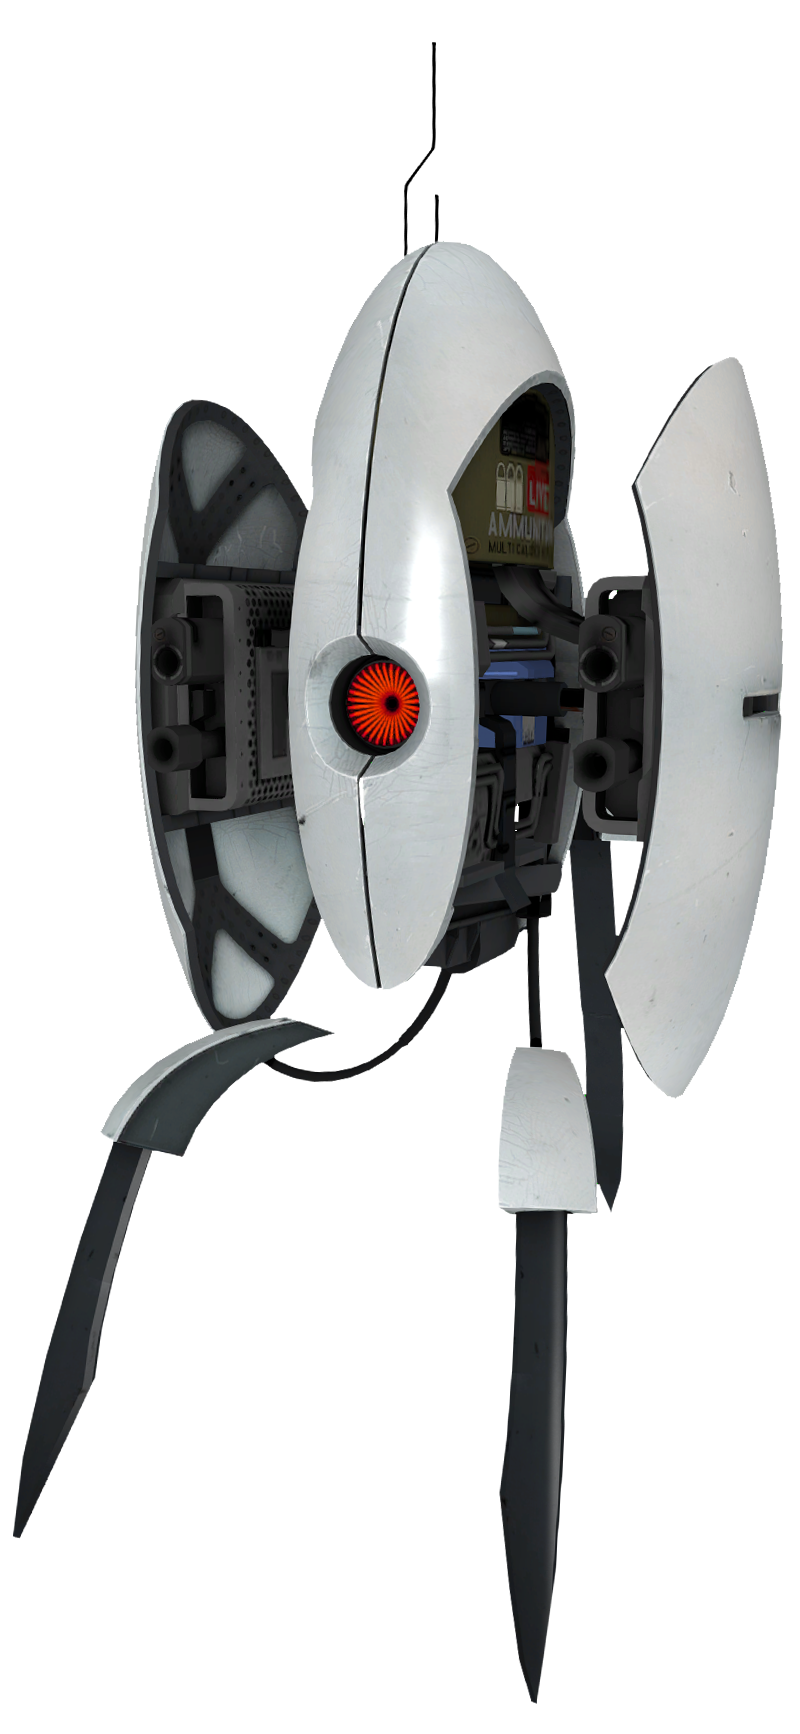
\includegraphics[width=0.6\linewidth]{irod_portal} 
		\caption{Portal Sentry Gun \cite{portal}}
		\label{fig:irod_portal}
	\end{minipage}
\end{figure}

Ezek olyan lövegek, amelyek a lábukon állva képesek voltak forogni, és ha az ellenség a látóterükbe jutott, akkor arra tüzet nyitottak. Nyilván játékokról van szó, tehát mindig azt hittem hogy ez csak a jövő technológiája, de nem sokkal később rá kellett jönnöm, hogy nagyon is valódiak. Ezután, mikor már egyetemre jártunk, egy barátommal egyre komolyabban kezdtünk beszélgetni arról, hogy esetleg mi is tudnánk egyet építeni. Végül az egyetemi éveim végére érve el is jött a tökéletes alkalom, hogy megvalósítsam régi álmomat. \\

A szentimentalitást félretéve, természetesen nem választottam volna ezt a témát, ha nem lenne a tanulmányaim szempontjából is releváns. Úgy gondolom, ez a projekt a mechatronika oktatás sok fontos elemét magában hordozza. A feladat a mechanikai konstrukcióval kezdődik és a CAD modellezéssel, amely a \textsl{gépészeti} oldalát hasznosítja a képzésünknek. Foglakozni kell a hardverrel, amihez \textsl{elektronikai} ismeretek szükségesek. Végül pedig a szoftvert kell lefejleszteni, ami \textsl{informatikai} szempontból érdekes. Ráadásul az egész beágyazott környezetben történik, ami miatt még relevánsabb az \textsl{intelligens beágyazott rendszerek} specializációmhoz. Véleményem szerint a projekt nehézsége és kihívása nem az egyes alfeladatokban rejlik, hanem az egész rendszer integrálásában, egymáshoz illesztésében. \\

Szintén fontosnak tartom megemlíteni, hogy a feladat lehetőséget ad megismerni és használni pár igen modern technológiát. A közelmúltban elérhetővé (és megfizethetővé) váltak civil felhasználásra a \textsl{3D nyomtatók}, valamint a fejlődés a \textsl{Deep Learning} algoritmusok terén nagyban befolyásolta a gépi látás szakterületét is. Többek között a célom, hogy jobban megismerkedjek ezekkel a módszerekkel, és alkalmazzam őket.\\

\begin{figure}[h!]
	\centering
	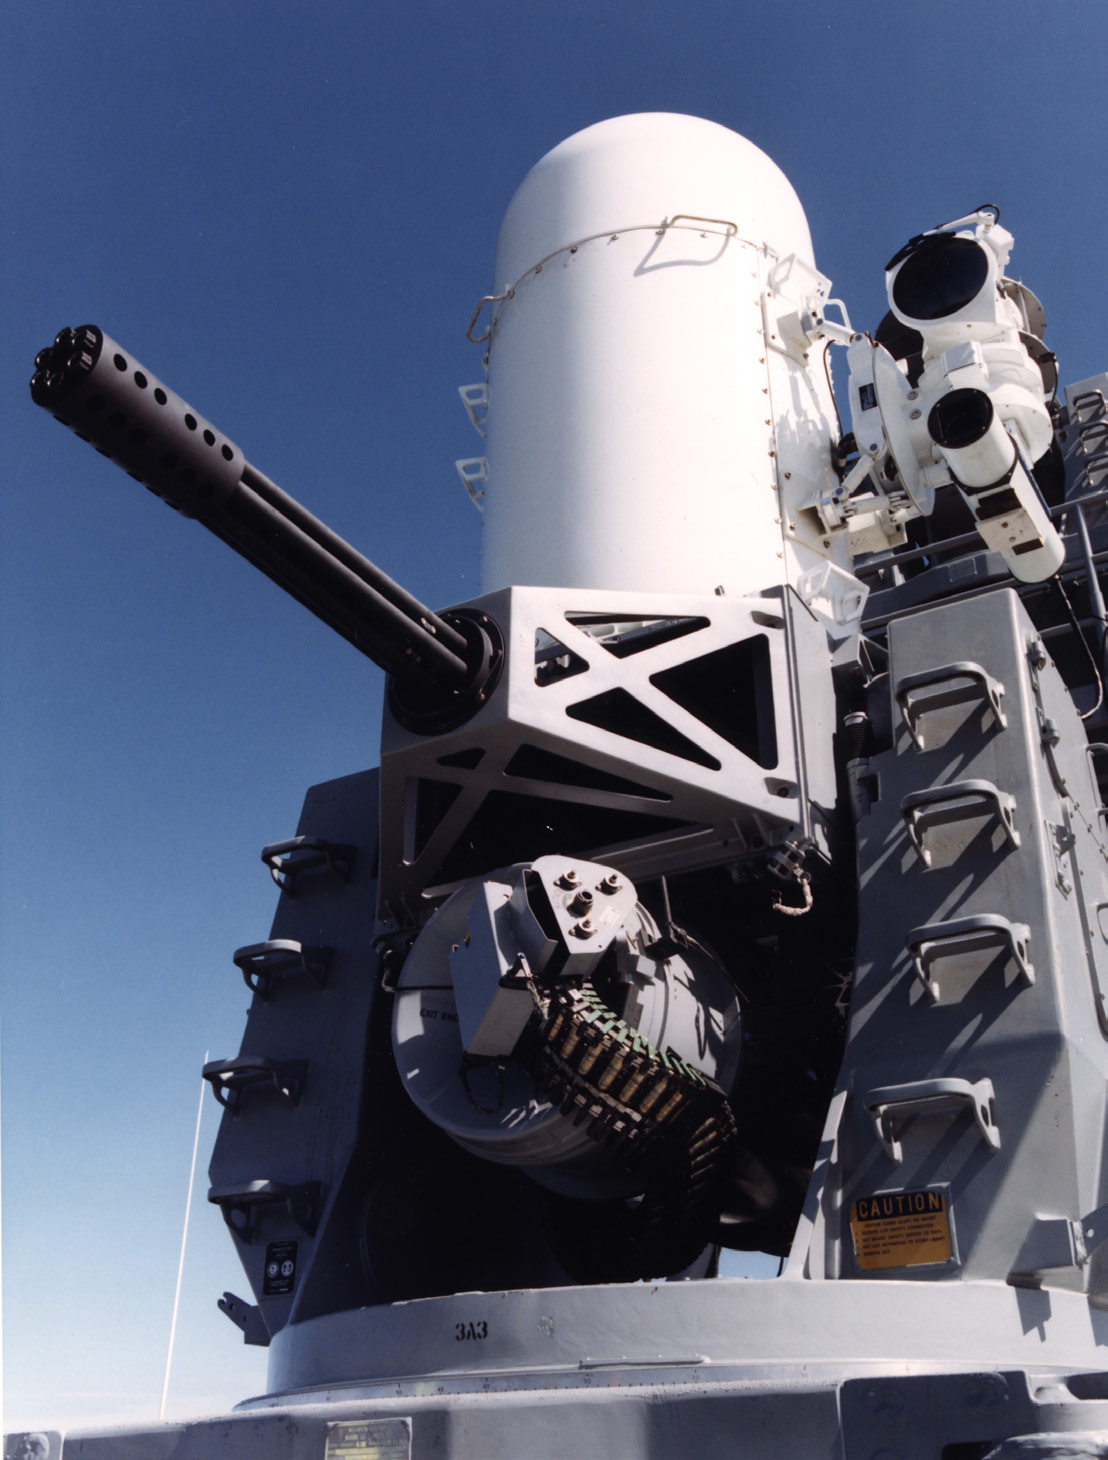
\includegraphics[width=.45\linewidth]{irod_phalanx} 
	\caption{Phalanx CIWS rendszer \cite{CIWS}}
	\label{fig:irod_phalanx}
\end{figure}

Mint manapság az ipar minden területén, így a fegyveriparban is egyre nagyobb mértékű a \textsl{digitalizáció} és az \textsl{automatizáció}. Ennek ékes példája a távolról irányítható fegyverrendszerek térnyerése, amelyeknek nagy előnye a fegyver és a tüzér egymástól való elkülönítése, aminek több előnye is van. Természetesen a legfontosabb és leginkább szembetűnő, hogy ezzel a módszerrel minimalizálható, vagy akár megszüntethető a saját embereink életének kockáztatása. Ezentúl olyan helyen is tudjuk használni ezeket az eszközöket, ahova egy tradicionális géppuskafészek telepítése nehézkes lenne, például mostoha természeti körülmények közé, egy torony tetejére, vagy akár egy hadihajó oldalára. Szintén egy nagy előny, hogy ezek az eszközök felszerelhetők több kezeléssegítő alegységgel, például hőkamerával vagy éjjellátóval. Majdnem minden, számottevő hadsereggel rendelkező országnak van saját fejlesztésű távirányított fegyverrendszere.\\

A következő lépés az \textsl{automatizálás}. Hiszen egyre erősebb hardverekkel rendelkezünk, egyre jobb algoritmusokat tudunk implementálni, és elértük az a szintet, hogy bizonyos helyzetekben a "gép" jobb munkát tud végezni, mint egy ember. Az első automatikus célzórendszerrel rendelkező légvédelmi gépágyú az amerikai \textsl{Phalanx CIWS} \cite{CIWS} az 1970-es években került kifejlesztésre, ezzel megszületett a "Lethal autonomous weapon (LAW)" kifejezés.\\

A technológiát érthető módon leggyakrabban védelmi célokra használják, sokszor légvédelemre. A gyakorlatban nagy szerepe van Dél-Korea és Izrael védelmében, ahol a rakétatámadások mindennapos veszélyt jelentenek. Offenzív célokra a gyakorlatban még csak rakéták célzására használnak automatikát, a "terminátor" jellegű gyilkos robotok még csak fejlesztési fázisban vannak.


\section{Kihívások és célkitűzések}

A hagyományos, ember által irányított biztonsági rendszerek, illetve manuálisan vezérelt fegyverek hatékonysága korlátozott. Az ember reakcióideje lassú lehet krízishelyzetben, különösen ha nagy sebességű, gyors reagálású, esetleg automatizált a célpont. További gyengesége az embernek, hogy hajlamos hibázni. A fáradtság, stressz, éhség, és rengeteg egyéb tényező kényszerítheti hibára. Ez szükségessé teszi egy olyan automata rendszer kifejlesztését, amely képes azonnal reagálni, felismerni a fenyegetéseket és pontosan célozni.\\

Az automatikus gépágyúk fejlesztése során számos technikai kihívás merül fel:\\

\textbf{Célpontok felismerése és követése:} A gépágyúnak gyorsan és pontosan kell érzékelnie és nyomon követnie mozgó célpontokat. Ez kihívást jelenthet változó fényviszonyok, mozgássebességek és környezeti zavaró tényezők mellett. \\

\textbf{Pontosság és reakcióidő:} A rendszernek gyorsan kell döntéseket hoznia, ugyanakkor elengedhetetlen a pontos célzás. A mechanikai mozgásvezérlés, a számítógépes látás és az elektronikai rendszerek szinkronizációja mind kritikus tényező a rendszer hatékonysága szempontjából. \\

\textbf{Környezetérzékenység:} Külső környezeti tényezők (pl. időjárás, akadályok, fényviszonyok) befolyásolhatják a rendszer működését, ezért a szoftvernek és a hardvernek \textsl{rugalmasnak} és \textsl{robusztusnak} kell lennie. A dolgozatom célja egy innovatív megoldás kidolgozása, amely eleget tesz a megszabott követelményeknek és megoldást nyújt a fenti problémákra. \\

\textbf{Kiemelt célok:}
\begin{list}{$\bullet$}{}
	\item Egy megbízható célpontfelismerési rendszer fejlesztése, amely változó környezeti feltételek mellett is képes hatékonyan működni.
	\item Egy stabil és erős mechanikai konstrukció tervezése, amely képes követni a szoftver utasításait.
	\item Egy olyan valós idejű szoftvervezérlési rendszer megalkotása, amely gyorsan reagál a célpontok mozgására és változására.
\end{list}

Összegezve tehát: \\

\textbf{Egy olyan automata gépágyú fejlesztése és megépítése, amely magabiztosan képes felismerni egy célpontot, követni azt, célozni, és tüzelni.}

\section{Korlátozások}

Természetesen tisztában kell lenni bizonyos korlátozásokkal a projekt elkészítése közben. Csupán két félévem van lefejleszteni, egyedül vagyok, és nincsen százmilliós büdzsém, mint az iparban hasonló kutatással foglalkozó csapatoknak. Ebből kifolyólag reálisan kell látni a helyzetet, és úgy meghatározni a követelményeket, hogy egy egyetemi hallgató számára is elérhető legyen. \\

A kamerarendszer például, amit a valós megoldásokban használnak, önmagában tízmilliós tétel szokott lenni. Sajnos az én megvalósításom valószínűleg nem fog működni sötétben, nagy távolságokban, vagy esőben, hiszen a költségvetésbe nem fér bele az éjjellátó, a hőkamera, az optikai zoom vagy több kamerából álló rendszer.\\

Nem áll rendelkezésemre korlátlanul se CNC gép, se fém 3D nyomtató, így a legtöbb alkatrészt műanyagból kell elkészítenem. Ez befolyásolhatja a szerkezet stabilitását, amit figyelembe kell venni a későbbiekben.\\

És végül fontos megemlíteni, hogy mivel valamilyen játékfegyvert kell majd használnom, ez befolyásolni fogja a gépágyú pontosságát, amit szintén figyelembe kell venni a tervezéskor és értékeléskor.\\


\pagebreak

\section{Erkölcsi nyilatkozat}
Az automata fegyverrendszer morális megítélése vitatott téma, ezért szeretném kijelenteni, hogy diplomamunkám, melynek címe \textsl{„Mikrovezérlő alapú autonóm fegyverrendszer tervezése és fejlesztése”}, kizárólag tanulmányi és mérnöki célokat szolgál. A dolgozatom keretében fejlesztett prototípus semmilyen formában nem szándékozik ösztönzi az erőszakos, káros vagy törvénysértő tevékenységeket. Fejlesztésem célja a technológiai kutatás, a mechatronikai és automatizálási rendszerek megismerése, illetve a gépi látás alkalmazásainak tanulmányozása. \\

Határozottan elhatárolódom bármilyen rosszindulatú felhasználástól, és hangsúlyozom, hogy a projekt eredményei nem használhatók fel ártalmas vagy illegális célokra. A munka során mindvégig tiszteletben tartottam az etikai irányelveket, és felelős mérnöki magatartást tanúsítottam. Az általam fejlesztett rendszer kizárólag oktatási, kutatási és technológiai demonstráció célját szolgálja.
